% --------------------------------------------------
%  TALLER DE INTRODUCCIÓN A LaTeX
%  https://github.com/mianfg/latex-intro
%
%  Sesión 1 -> Presentación
%
%  Autor: Miguel Ángel Fernández Gutiérrez, @mianfg
%  Fecha: 20 febrero, 2019
% --------------------------------------------------

% Tipo de documento (presentación)
\documentclass[10pt, xcolor=table]{beamer}

% Cargar el tema
\usetheme{metropolis}

%  __________
% |          |
% | Paquetes |
% |__________|

% Paquetes de idioma
\usepackage[utf8]{inputenc}
\usepackage[spanish, es-tabla, es-lcroman, es-noquoting]{babel}

% Paquete para código fuente
% LISTINGS
\usepackage{listings}
\usepackage{lipsum}
\usepackage{courier}

% Colores para los bloques de código
\definecolor{codegreen}{rgb}{0,0.6,0}
\definecolor{codegray}{rgb}{0.5,0.5,0.5}
\definecolor{codepurple}{rgb}{0.58,0,0.82}
\definecolor{backcolour}{rgb}{0.95,0.95,0.92}
\lstdefinestyle{mystyle}{
	backgroundcolor=\color{backcolour},   
	commentstyle=\color{codegreen},
	keywordstyle=\color{blue},
	numberstyle=\tiny\color{codegray},
	stringstyle=\color{codepurple},
	basicstyle=\footnotesize\ttfamily,
	breakatwhitespace=false,         
	breaklines=true,                 
	captionpos=b,                    
	keepspaces=true,                 
	numbers=left,                    
	numbersep=5pt,                  
	showspaces=false,                
	showstringspaces=false,
	showtabs=false,                  
	tabsize=4
}
\lstset{style=mystyle}

% Paquete de numeración en Beamer
\usepackage{appendixnumberbeamer}

% Paquete de uso para plantilla
\usepackage{booktabs}
\usepackage[scale=2]{ccicons}

% Paquete para controlar espacios
\usepackage{xspace}
\newcommand{\themename}{\textbf{\textsc{metropolis}}\xspace}

% Paquetes para matemáticas
\usepackage{amsmath}    % Paquete básico de matemáticas
\usepackage{amsthm}     % Teoremas
\usepackage{mathrsfs}   % Fuente para ciertas letras utilizadas en matemáticas

% Paquetes para fuentes
\usepackage{newpxtext, newpxmath}   % Fuente similar a Palatino
\usepackage{FiraSans}               % Fuente sans serif
\usepackage[T1]{fontenc}
\usepackage[italic]{mathastext}     % Utiliza la fuente del documento
                                    % en los entornos matemáticos

%  ________________________
% |                        |
% | Configuración del tema |
% |________________________|

% Configuración básica del tema
\metroset{
  % tema oscuro ('dark') o claro ('light'). No tiene efecto al usar la
  % paleta de colores más adelante
  background=light,
  % 'none' para eliminar la diapositiva inicial de cada sección
  sectionpage=progressbar,
  % 'progressbar' o 'simple' para añadir una diapositiva inicial a cada subsección
  subsectionpage=none,
  % contador de página: 'none', 'counter' o 'fraction'
  numbering=none,
  % barra de progreso: 'none', 'head', 'frametitle' o 'foot'
  progressbar=frametitle,
  % fondo de los bloques estilo teorema: 'transparent' o 'fill'
  block=fill,
}

% Paleta de colores
\definecolor{accent}{HTML}{009688}
\colorlet{darkaccent}{accent!70!black}
\definecolor{foreground}{RGB}{0, 0, 0}
\definecolor{background}{RGB}{255, 255, 255}

% Insertar los colores en el tema
\setbeamercolor{normal text}{fg=foreground, bg=background}
\setbeamercolor{alerted text}{fg=darkaccent, bg=background}
\setbeamercolor{example text}{fg=foreground, bg=background}
\setbeamercolor{frametitle}{fg=background, bg=accent}

\setbeamercolor{headtitle}{fg=background!70!accent,bg=accent!90!foreground}
\setbeamercolor{headnav}{fg=background,bg=accent!90!foreground}
\setbeamercolor{section in head/foot}{fg=background,bg=accent}

\defbeamertemplate*{headline}{miniframes theme no subsection}{
  % Caja para mostrar título y autor encima de cada diapositiva
  % Nosotros no 
  %% \begin{beamercolorbox}[ht=2.5ex,dp=1.125ex,
  %%     leftskip=.3cm,rightskip=.3cm plus1fil]{headtitle}
  %%   {\usebeamerfont{title in head/foot}\insertshorttitle}
  %%   \hfill
  %%   \leavevmode{\usebeamerfont{author in head/foot}\insertshortauthor}
  %% \end{beamercolorbox}
  %% \begin{beamercolorbox}[colsep=1.5pt]{upper separation line head}
  %% \end{beamercolorbox}

  % Caja para mostrar navegación encima de cada diapositiva
  \begin{beamercolorbox}{headnav}
    \vskip2pt\insertnavigation{\paperwidth}\vskip2pt
  \end{beamercolorbox}
  \begin{beamercolorbox}[colsep=1.5pt]{lower separation line head}
  \end{beamercolorbox}
}

%  _________
% |         |
% | Ajustes |
% |_________|

% Fijar tabla a posición
\usepackage{array}
\newcolumntype{L}[1]{>{\raggedright\let\newline\\\arraybackslash\hspace{0pt}}m{#1}}
\newcolumntype{C}[1]{>{\centering\let\newline\\\arraybackslash\hspace{0pt}}m{#1}}
\newcolumntype{R}[1]{>{\raggedleft\let\newline\\\arraybackslash\hspace{0pt}}m{#1}}

%  ________
% |        |
% | Título |
% |________|

\title{Algoritmos voraces (\emph{greedy})}
\subtitle{Algorítmica. \alert{Práctica 3}}
\date{}
\author{Celia Arias Martínez\\Miguel Ángel Fernández Gutiérrez\\Sergio Quijano Rey\\Lucía Salamanca López\\[4pt]\footnotesize{segfault}}
\titlegraphic{\hfill
\includegraphics[width=2.5cm]{ugrlogo-dark.pdf}}

%  ___________
% |           |
% | Documento |
% |___________|

\begin{document}

\maketitle

\begin{frame}{Contenidos}
	\setbeamertemplate{section in toc}[sections numbered]
	\tableofcontents[]
\end{frame}


\section{Introducción}

\begin{frame}{Objetivo}
Apreciar la utilidad de los métodos voraces (\textit{greedy}) para resolver problemas de forma muy eficiente, en algunos obteniendo soluciones óptimas y en otros aproximaciones. Para ello realizamos:
\begin{itemize}
	\item \textbf{Problema común:} problema del viajante de comercio (TSP).
	\item \textbf{Problema asignado:} trabajadores y tareas (\emph{worker}).
\end{itemize}

\end{frame}

\section{Problema del viajante de comercio (TSP)}

\begin{frame}{Problema común}
\begin{center}
\textbf{\large{Travelling Salesman Problem (TSP)}}
\end{center}
Dado un conjunto de ciudades y una matriz con las distancias entre todas ellas, un viajante debe recorrer todas las ciudades exactamente una vez, regresando al punto de partida, de forma tal que la distancia recorrida sea mínima. 

Formalmente: dado un grafo \textit{G}, conexo y ponderado, se trata de hallar el \textit{ciclo hamiltoniano} de mínimo peso de ese grafo.
\end{frame}

\begin{frame}{Enfoque 1: por cercanía}
Dada una ciudad inicial \textit{$v_0$}, se agrega como ciudad siguiente aquella \textit{$v_i$} (no incluída en el circuito) que se encuentre más cercana a \textit{$v_0$}. El procedimiento se repite hasta que todas las ciudades se hayan visitado.
\end{frame}
\begin{frame}{Enfoque 1: por cercanía}
\begin{center}
\textbf{\large{PASOS}}
\end{center}
\begin{enumerate}
		\item Partimos del nodo $0$
		\item Encontramos, en el vector de nodos disponibles, el más cercano al anterior.
		\item Eliminamos el escogido del vector.
		\item Repetimos los pasos anteriores con los nuevos nodos hasta que el vector se quede vacío.
		\item Finalmente devuelve el camino.
	\end{enumerate}
\end{frame}
\begin{frame}{Enfoque 1: por cercanía}
Para este enfoque usamos:
\begin{itemize}
	\item Un \emph{struct} \texttt{Point}, que tiene una coordenada \texttt{x}, una coordenada \texttt{y}, y una función \texttt{distancia} para calcular la distancia entre dos \texttt{Point}.
	\item Una función \texttt{get\_best\_solution}, que calcula la solución especificada anteriormente. Para ello, hace uso de:
	\begin{itemize}
		\item \texttt{road}, un vector donde se almacenan las soluciones parciales, es decir, las que resultan de añadir un nodo al recorrido.
		\item \texttt{points\_left}, vector donde almacenamos los nodos que nos quedan por recorrer.
	\end{itemize}
\end{itemize}
\end{frame}

\begin{frame}{Enfoque 1: por cercanía}
Guardamos en \texttt{points\_left} todos los nodos y en \texttt{road} el primer punto, que podemos asumir que es el primero. 

Mientras que el vector \texttt{points\_left} no esté vacío calculamos la distancia de todos esos nodos al último Punto de \texttt{road} y añadimos el nodo que esté a la menor distancia, borrándolo de \texttt{points\_left}.
\end{frame}

\begin{frame}{Enfoque 1: por cercanía. \normalfont{Análisis empírico}}
\begin{itemize}
	\item \textbf{Tamaños de prueba:} desde 100 hasta 4000 ciudades, incremento de 200.
	\item Cada iteración la repetimos 100 veces y hacemos la media, con el fin de eliminar peores y mejores casos.
\end{itemize}
\end{frame}

\begin{frame}[fragile]{Enfoque 1: por cercanía. \normalfont{Análisis empírico}}
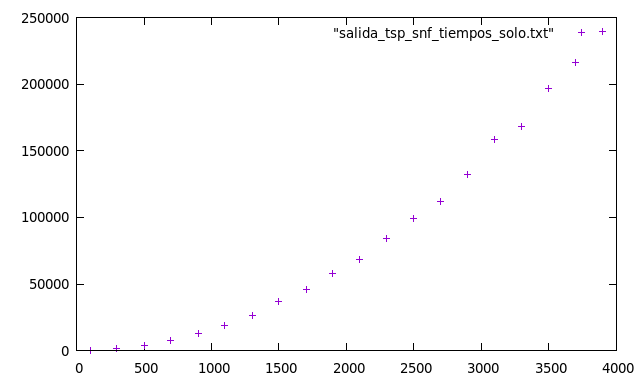
\includegraphics[width=\textwidth]{../Graficas/graficastsp/snfTiempo.png}
\begin{center}
	\footnotesize{Datos empíricos para viajante de comercio versión cercanía, tiempo}
\end{center}
\end{frame}

\begin{frame}[fragile]{Enfoque 1: por cercanía. \normalfont{Análisis empírico}}
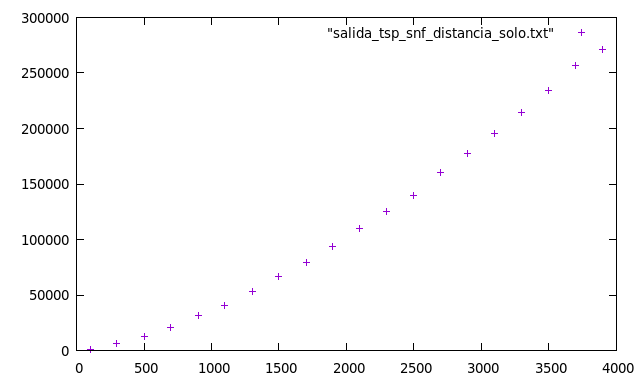
\includegraphics[width=\textwidth]{../Graficas/graficastsp/snfDistancia.png}
\begin{center}
	\footnotesize{Datos empíricos para viajante de comercio versión cercanía, distancia}
\end{center}
\end{frame}

\begin{frame}{Enfoque 2: por inserción}
Se comienza con un recorrido parcial y luego se extiende insertando las ciudades restantes mediante algún criterio de tipo voraz: insertando los nodos de modo que el recorrido sea mínimo.
\end{frame}

\begin{frame}{Enfoque 2: por inserción}
\begin{center}
\textbf{\large{PASOS}}
\end{center}
\begin{enumerate}
		\item Partimos de tres nodos: 
		\begin{itemize}
			\item El que está más al \textit{Norte}.
			\item El que está más al \textit{Este}. 
			\item El que está más al \textit{Oeste}.
		\end{itemize}
		\item Partiendo de este camino añadimos el punto de forma que la distancia del nuevo camino sea mínima.
		\item Repetimos esto sucesivamente hasta que tengamos todos los puntos.
		\item Finalmente devuelve el camino.
	\end{enumerate}
\end{frame}

\begin{frame}{Enfoque 2: por inserción}
Hacemos uso de:
\begin{itemize}
	\item \texttt{candidates} es el vector con los nodos que faltan por insertar. 
	\item \texttt{road} es el vector con la solución parcial. 
	\item \texttt{most\_north} es el nodo más al norte.
	\item \texttt{most\_west} es el nodo más al oeste.
	\item \texttt{most\_east} es el nodo más al este.
	\item \texttt{get\_best\_candidate} es una función auxiliar que dado un camino y un vector de candidatos devuelve un vector con la posición del punto óptimo y dónde queremos insertarlo en el camino. 
\end{itemize}
\end{frame}

\begin{frame}{Enfoque 2: por inserción}
En la nueva función \texttt{get\_best\_solution}, primero calculamos e insertamos en \texttt{road} los nodos más al norte, este y oeste, para que se queden dentro los máximos nodos posibles. Mientras que \texttt{candidates} no sea vacío calculamos el nodo y la posición con los cuales la distancia que tenemos que recorrer aumenta lo mínimo posible al añadir un nodo, y lo insertamos en \texttt{road}, quitándolo de \texttt{candidates}.
\end{frame}

\begin{frame}{Enfoque 2: por inserción. \normalfont{Análisis empírico}}
\begin{itemize}
	\item \textbf{Tamaños de prueba:} desde 3 hasta 200 ciudades, con incremento de 10.
	\item Cada iteración la repetimos 100 veces y hacemos la media, con el fin de eliminar peores y mejores casos.
\end{itemize}
\end{frame}

\begin{frame}[fragile]{Enfoque 2: por inserción. \normalfont{Análisis empírico}}
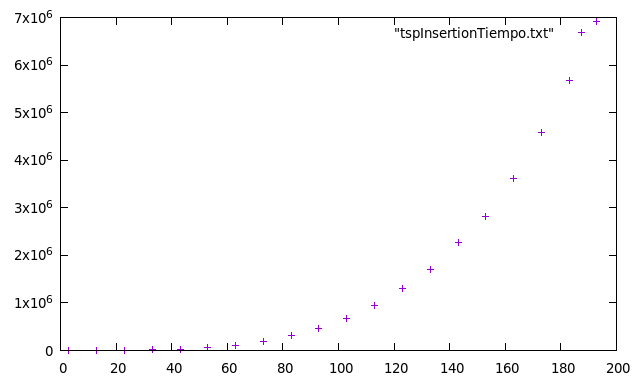
\includegraphics[width=\textwidth]{../Graficas/graficastsp/insertionTiempo.png}
\begin{center}
	\footnotesize{Datos empíricos para viajante de comercio versión inserción, tiempo}
\end{center}
\end{frame}

\begin{frame}[fragile]{Enfoque 2: por inserción. \normalfont{Análisis empírico}}
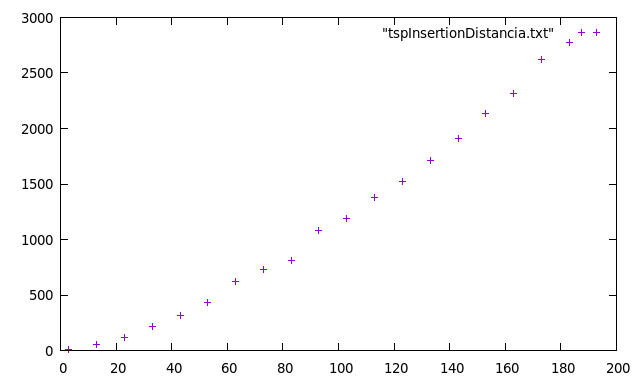
\includegraphics[width=\textwidth]{../Graficas/graficastsp/insertionDistancia.png}
\begin{center}
	\footnotesize{Datos empíricos para viajante de comercio versión inserción, distancia}
\end{center}
\end{frame}


\begin{frame}{Enfoque 3: por perturbaciones}
Este enfoque, de nuevo \emph{greedy}, dado un recorrido, realiza las perturbaciones indicadas por un parámetro para intentar mejorarlo.
\end{frame}

\begin{frame}{Enfoque 3: por perturbaciones}
\begin{center}
\textbf{\large{PASOS}}
\end{center}
\begin{enumerate}
	\item Calculamos la solución dada por el algoritmo SNF.
	\item Calculamos el nodo respecto el que tenemos que perturbar.
	\item Perturbamos y vemos la ganancia del camino.
	\item Si la ganancia es mejor se cambia el camino.
	\item Se devuelve el camino.
\end{enumerate}
\end{frame}

\begin{frame}{Enfoque 3: por perturbaciones}
Hacemos uso de:

\begin{itemize}
	\item \texttt{points} es un vector con los nodos dados. 
	\item \texttt{perturbations} es el número de perturbaciones que aplicamos al algoritmo. 
	\item \texttt{get\_snf\_solution} es una función auxiliar que calcula según el algoritmo por cercanía una solución al conjunto de puntos.
	\item \texttt{get\_worst\_node} es una función auxiliar que calcula el nodo tal que según el recorrido actual su distancia al siguiente punto es la mayor.
	\item \texttt{perturbate} es una función auxiliar que encuentra un camino diferente que haga que el peor nodo mejore y sobrescribe el camino actual.
\end{itemize}
\end{frame}

\begin{frame}{Enfoque 3: por perturbaciones}
Primero calculamos una solución inicial con el algoritmo de \emph{cercanía}. Después calculamos el peor nodo de ese recorrido e intentamos encontrar otra combinación de nodos que mejore ese nodo en concreto. Este proceso lo repetimos tantas veces como \texttt{perturbations} indique. 
\end{frame}

\begin{frame}{Enfoque 3: por perturbaciones. \normalfont{Análisis empírico}}
\begin{itemize}
	\item \textbf{Tamaños de prueba:} desde 10 hasta 200 ciudades, con incremento de 20.
	\item Cada iteración la repetimos 100 veces y hacemos la media, con el fin de eliminar peores y mejores casos.
\end{itemize}
\end{frame}

\begin{frame}[fragile]{Enfoque 3: por perturbaciones. \normalfont{Análisis empírico}}
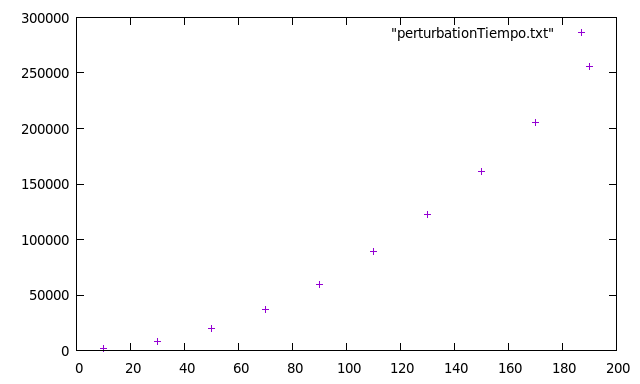
\includegraphics[width=\textwidth]{../Graficas/graficastsp/perturbationTiempo.png}
\begin{center}
	\footnotesize{Datos empíricos para viajante de comercio versión perturbaciones, tiempo}
\end{center}
\end{frame}

\begin{frame}[fragile]{Enfoque 3: por perturbaciones. \normalfont{Análisis empírico}}
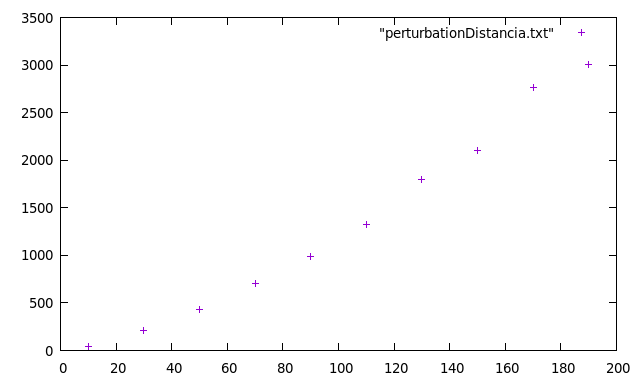
\includegraphics[width=\textwidth]{../Graficas/graficastsp/perturbationDistancia.png}
\begin{center}
	\footnotesize{Datos empíricos para viajante de comercio versión perturbaciones, distancia}
\end{center}
\end{frame}

\begin{frame}[fragile]{Comparación de enfoques}
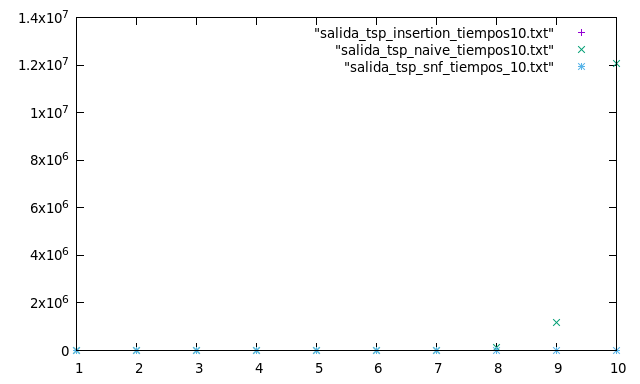
\includegraphics[width=\textwidth]{../Graficas/graficastsp/tiempo3.png}
\begin{center}
	\footnotesize{Contraste de datos empíricos: tiempo}
\end{center}
\end{frame}

\begin{frame}[fragile]{Comparación de enfoques}
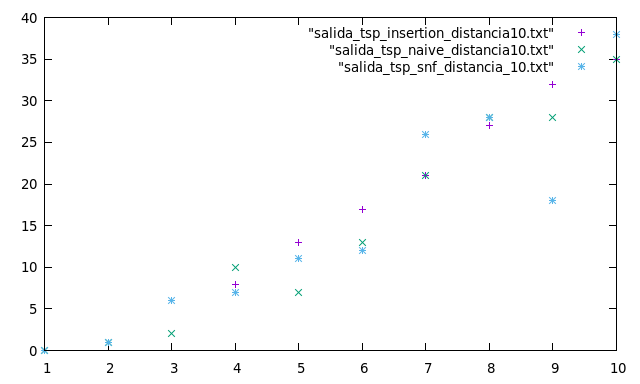
\includegraphics[width=\textwidth]{../Graficas/graficastsp/distancia3.png}
\begin{center}
	\footnotesize{Contraste de datos empíricos: distancia}
\end{center}
\end{frame}

\begin{frame}[fragile]{Comparación de enfoques}
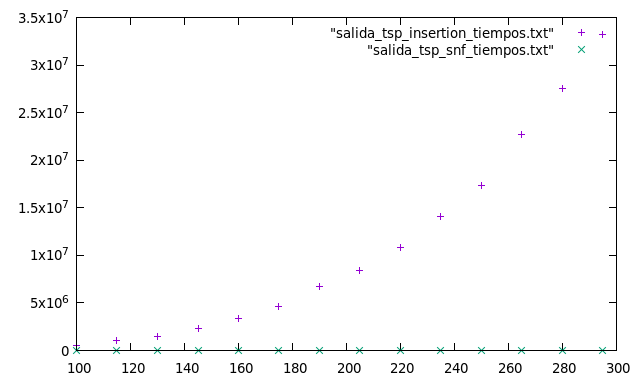
\includegraphics[width=\textwidth]{../Graficas/graficastsp/tiempo2.png}
\begin{center}
	\footnotesize{Contraste de datos empíricos (cercanía e inserción): tiempo}
\end{center}
\end{frame}

\begin{frame}[fragile]{Comparación de enfoques}
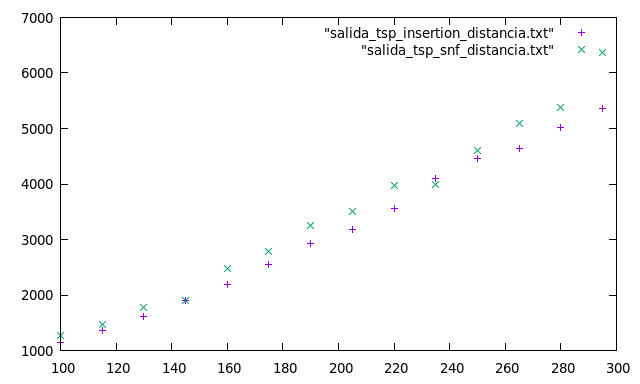
\includegraphics[width=\textwidth]{../Graficas/graficastsp/distancia2.png}
\begin{center}
	\footnotesize{Contraste de datos empíricos (cercanía e inserción): distancia}
\end{center}
\end{frame}

\begin{frame}[fragile]{Comparación de enfoques}
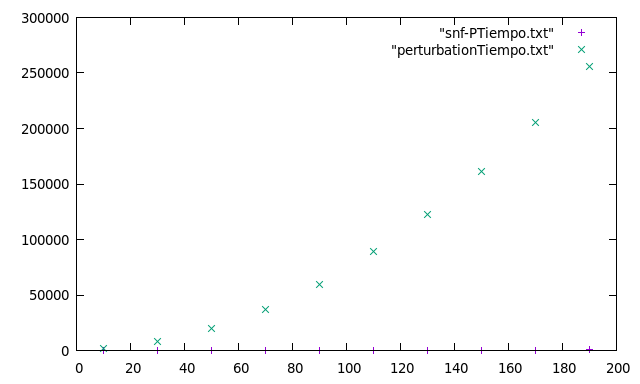
\includegraphics[width=\textwidth]{../Graficas/graficastsp/TiempoC-P.png}
\begin{center}
	\footnotesize{Contraste de datos empíricos (cercanía y perturbaciones): tiempo}
\end{center}
\end{frame}

\begin{frame}[fragile]{Comparación de enfoques}
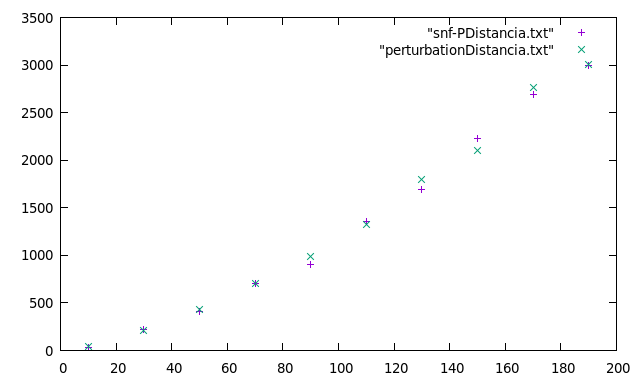
\includegraphics[width=\textwidth]{../Graficas/graficastsp/DistanciaC-P.png}
\begin{center}
	\footnotesize{Contraste de datos empíricos (cercanía y perturbaciones): distancia}
\end{center}
\end{frame}

\section{Asignación de tareas (\emph{worker})}

\begin{frame}{Problema asignado}
\begin{center}
\textbf{\large{Problema de la asignación de tareas}}
\end{center}
Supongamos que disponemos de \emph{n} trabajadores y \emph{n} tareas. Sea $\text{\sffamily \emph{c}}_\text{\sffamily \emph{ij}} > \text{\sffamily 0}$ el coste de asignarle la tarea \emph{j} al trabajador \emph{i}. Una asignación válida es aquella en la que a cada trabajador le corresponde una tarea y cada tarea la realiza un trabajador diferente. Dada una asignación válida, definimos el coste de dicha asignación como la suma total de los costes individuales. Diseñe un algoritmo voraz para obtener una asignación de tareas a trabajadores óptima.
\end{frame}

\begin{frame}{Notación}
Usaremos la siguiente notación:
\begin{itemize}
	\item $n$ es el \textbf{número de trabajadores}, que coincide con el \textbf{número de tareas}.
	\item $C$ es la \textbf{matriz de costes}, de tamaño $n\times n$, en el que el elemento $c_{ij}$ de la matriz es el coste de asignar al trabajador $i$ la tarea $j$.
	\item $a$ es el \textbf{vector de asignaciones}, de tamaño $n$. El trabajo asignado al trabajador $i$ estará contenido en el elemento $a_i$ del vector.
	\item $W_a$ es el coste de una cierta asignación $a$. Se calcula mediante:
	$$ W_a = \sum_{i=0}^{n-1} c_{i,a_i}$$
\end{itemize}
\end{frame}

\begin{frame}{Enfoque 1: inserción}
\begin{center}
	(1)
\end{center}
\begin{table}[h]
\centering
\begin{tabular}{c}
$C = \left(\begin{matrix}\textbf{2}&4&3\\1&4&2\\2&7&5\\\end{matrix}\right)\begin{matrix}\leftarrow\\\\\\\end{matrix}$\\
$a=\{0,\;,\;\}$\\
$d=\{\text{T},\text{T},\text{T}\}$\\
\end{tabular}
\end{table}
\end{frame}

\begin{frame}{Enfoque 1: inserción}
\begin{center}
	(2)
\end{center}
\begin{table}[h]
\centering
\begin{tabular}{c}
$C = \left(\begin{matrix}\textcolor{red}{2}&4&3\\\textcolor{red}{1}&4&2\\\textcolor{red}{2}&7&5\\\end{matrix}\right)\begin{matrix}\leftarrow\\\\\\\end{matrix}$\\
$a=\{0,\;,\;\}$\\
$d=\{\text{\textcolor{red}{F}},\text{T},\text{T}\}$\\
\end{tabular}
\end{table}
\end{frame}

\begin{frame}{Enfoque 1: inserción}
\begin{center}
	(3)
\end{center}
\begin{table}[h]
\centering
\begin{tabular}{ccc}
$C = \left(\begin{matrix}\textcolor{red}{2}&4&3\\\textcolor{red}{1}&4&\textbf{2}\\\textcolor{red}{2}&7&5\\\end{matrix}\right)\begin{matrix}\\\leftarrow\\\\\end{matrix}$&&$C = \left(\begin{matrix}\textcolor{red}{2}&4&\textcolor{red}{3}\\\textcolor{red}{1}&4&\textcolor{red}{2}\\\textcolor{red}{2}&7&\textcolor{red}{5}\\\end{matrix}\right)\begin{matrix}\\\leftarrow\\\\\end{matrix}$\\
$a=\{0,2,\;\}$ && $a=\{0,2,\;\}$\\
$d=\{\text{\textcolor{red}{F}},\text{T},\text{T}\}$&&$d=\{\text{\textcolor{red}{F}},\text{T},\text{\textcolor{red}{F}}\}$\\
\end{tabular}
\end{table}
\end{frame}

\begin{frame}{Enfoque 1: inserción}
Este enfoque se traduce en un código que comprende las siguientes funciones:

\begin{itemize}
	\item \texttt{get\_best\_solution}, una función para calcular la asignación especificada anteriormente.
	\item \texttt{find\_best\_task}, una función auxiliar para calcular la mejor tarea que se encuentre disponible (haciendo uso de un vector de disponibles, \texttt{available}), de un conjunto de tareas
\end{itemize}
\end{frame}

\begin{frame}{Enfoque 1: inserción. \normalfont{Análisis empírico}}
\begin{itemize}
	\item \textbf{Tamaños de prueba:} desde 100 hasta 400 trabajadores, con incremento de 200.
	\item Cada iteración la repetimos 100 veces y hacemos la media, con el fin de eliminar peores y mejores casos.
\end{itemize}
\end{frame}

\begin{frame}[fragile]{Enfoque 1: inserción. \normalfont{Análisis empírico}}
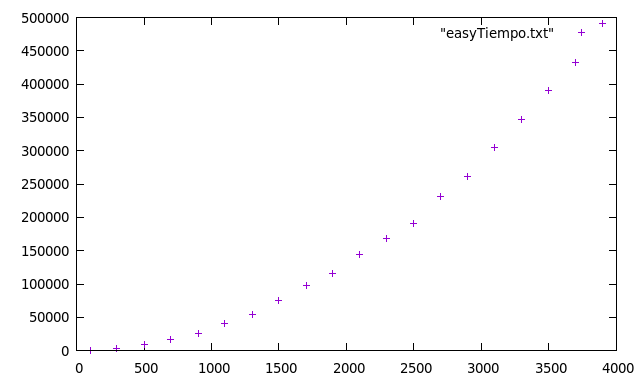
\includegraphics[width=\textwidth]{../Graficas/graficasWorker/easyTiempo.png}
\begin{center}
	\footnotesize{Datos empíricos para asignación de tareas versión inserción, tiempo}
\end{center}
\end{frame}

\begin{frame}[fragile]{Enfoque 1: inserción. \normalfont{Análisis empírico}}
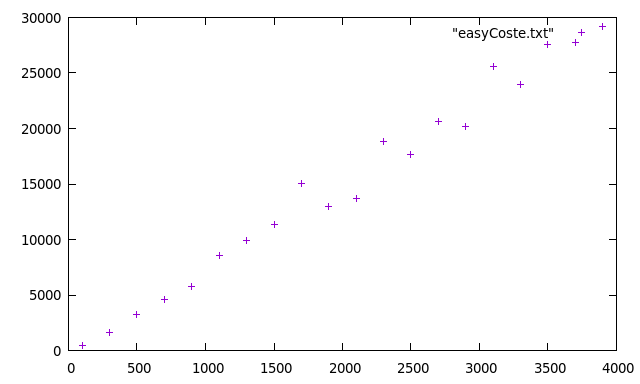
\includegraphics[width=\textwidth]{../Graficas/graficasWorker/easyCoste.png}
\begin{center}
	\footnotesize{Datos empíricos para asignación de tareas versión inserción, coste}
\end{center}
\end{frame}

\begin{frame}{Enfoque 2: permutaciones}
Este algoritmo consiste en, partiendo de una asignación, ir modificándola hasta encontrar una mejor, es decir, con una \textbf{ganancia} positiva.
\end{frame}

\begin{frame}{Enfoque 2: permutaciones}
\begin{center}
	(1)
\end{center}
Buscamos elemento con mayor coste de todas las asignaciones: $a_m$, donde $m$ es la posición del elemento en el vector $a$ de asignaciones.
\end{frame}

\begin{frame}{Enfoque 2: permutaciones}
\begin{center}
	(2)
\end{center}
Vamos permutando con $a_m$:
$$a'_0=\{a_m, a_1, ..., a_{m-1}, a_0, a_{m+1}, ..., a_{n-1}\},$$$$a'_1 = \{a_0, a_m, a_2, ..., a_{m-1}, a_1, a_{m+1}, a_{n-1}\}, ...$$
Tomamos la que tenga mayor \textbf{ganancia} ($p$ con $W_{a'_p}$ menor).
\end{frame}

\begin{frame}{Enfoque 2: permutaciones}
\begin{center}
	(3)
\end{center}
Repetimos número \textbf{arbitrario} de veces: cada iteración, obtenemos solución mejor, o misma solución.
\end{frame}

\begin{frame}{Enfoque 2: permutaciones}
Podemos partir de la asignación que proporciona el enfoque por \emph{inserción}.
\end{frame}

\begin{frame}{Enfoque 2: permutaciones}
Este enfoque se traduce en un código que comprende las siguientes funciones:

\begin{itemize}
	\item \texttt{get\_best\_solution}, de nuevo nuestra función principal para resolver el problema.
	\item \texttt{find\_worst\_worker}, una función auxiliar para encontrar el trabajador que tiene la \emph{peor tarea asignada}, es decir, el que tiene mayor costo (1).
	\item \texttt{find\_best\_permutation}, una función auxiliar que, de entre todas las permutaciones posibles, encuentra la que tiene una ganancia mayor (2).
	\item \texttt{permutate}, una función auxiliar que efectúa la permutación, es decir, modifica el vector $a$ de asignaciones para efectuar el intercambio encontrado.
\end{itemize}
\end{frame}

\begin{frame}{Enfoque 2: permutaciones. \normalfont{Análisis empírico}}
\begin{itemize}
	\item \textbf{Tamaños de prueba:} desde 1 hasta 100 trabajadores, con incremento de 10.
	\item Cada iteración la repetimos 100 veces y hacemos la media, con el fin de eliminar peores y mejores casos.
\end{itemize}
\end{frame}

\begin{frame}[fragile]{Enfoque 2: permutaciones. \normalfont{Análisis empírico}}
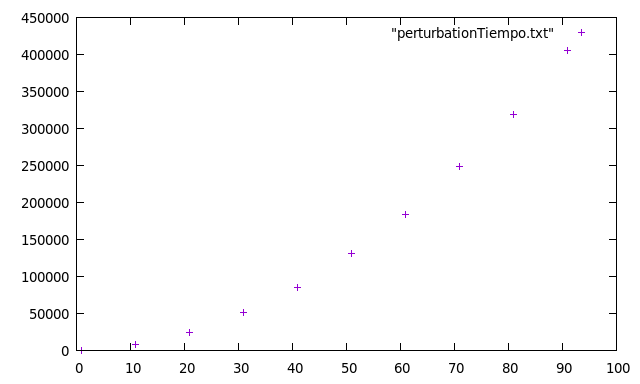
\includegraphics[width=\textwidth]{../Graficas/graficasWorker/perturbationTiempo.png}
\begin{center}
	\footnotesize{Datos empíricos para asignación de tareas versión permutaciones, tiempo}
\end{center}
\end{frame}

\begin{frame}[fragile]{Enfoque 2: permutaciones. \normalfont{Análisis empírico}}
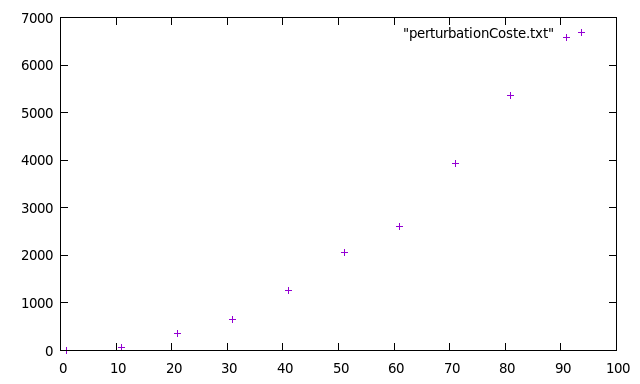
\includegraphics[width=\textwidth]{../Graficas/graficasWorker/perturbationCoste.png}
\begin{center}
	\footnotesize{Datos empíricos para asignación de tareas versión permutaciones, coste}
\end{center}
\end{frame}

\begin{frame}{Comparación de enfoques}
Ambos enfoques son \emph{greedy}, e intentan acercarse a la mejor solución.

$$C=\left(\begin{matrix}1&2\\2&10\end{matrix}\right)$$

\begin{center}
	\footnotesize{Coste asignación por inserción: 11\\Coste óptimo: 4}
\end{center}

Enfoque con permutaciones nos conduciría a solución óptima en una iteración.
\end{frame}

\begin{frame}{Comparación de enfoques}
Enfoque con permutaciones es especialmente interesante cuando partimos de una cantidad muy grande de datos, ya que tener una estimación inicial puede ser complicado.

Podemos partir de asignación cualquiera y mejorarla con sucesivas iteraciones.
\end{frame}

\begin{frame}[fragile]{Comparación de enfoques}
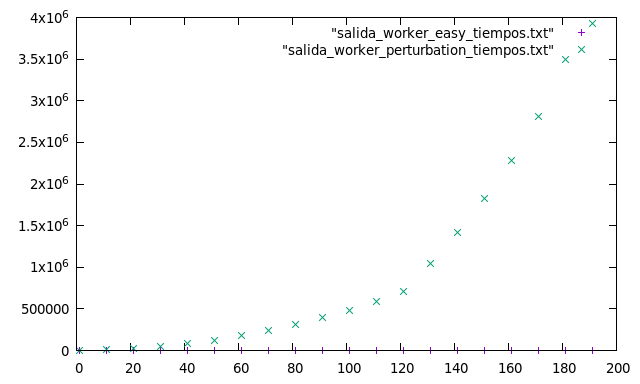
\includegraphics[width=\textwidth]{../Graficas/graficasWorker/tiempos2.png}
\begin{center}
	\footnotesize{Contraste de datos empíricos (inserción y permutaciones): tiempo}
\end{center}
\end{frame}


\begin{frame}[fragile]{Comparación de enfoques}
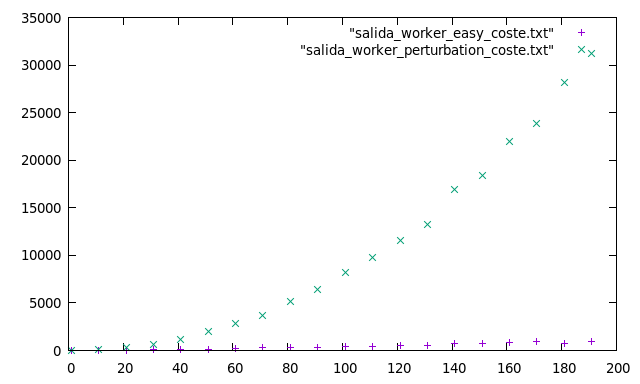
\includegraphics[width=\textwidth]{../Graficas/graficasWorker/coste2.png}
\begin{center}
	\footnotesize{Contraste de datos empíricos (inserción y permutaciones): coste}
\end{center}
\end{frame}

\begin{frame}[fragile]{Comparación de enfoques}
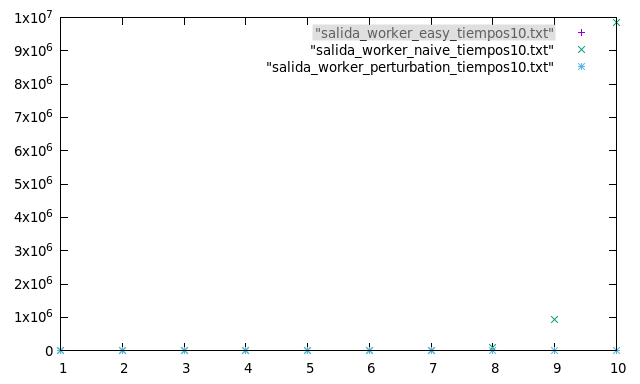
\includegraphics[width=\textwidth]{../Graficas/graficasWorker/tiempos3.png}
\begin{center}
	\footnotesize{Contraste de datos empíricos (inserción, permutaciones y fuerza bruta): tiempo}
\end{center}
\end{frame}

\begin{frame}[fragile]{Comparación de enfoques}
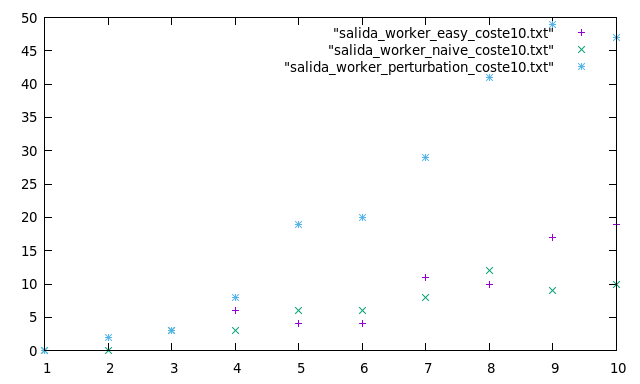
\includegraphics[width=\textwidth]{../Graficas/graficasWorker/coste3.png}
\begin{center}
	\footnotesize{Contraste de datos empíricos (inserción, permutaciones y fuerza bruta): coste}
\end{center}
\end{frame}

\section{Conclusiones}

\begin{frame}{Conclusiones}
Hemos aprendido a crear algoritmos voraces para resolver problemas que, en su versión en fuerza bruta, tienen una complejidad muy elevada, con diversos \textbf{enfoques \emph{greedy}}.

Hay problemas en el que encontrar la solución óptima es muy costoso. Podemos entonces ``acercarnos'' a ella mediante los \textbf{algoritmos \emph{greedy}}, y especialmente haciendo uso de enfoques con \textbf{permutaciones} a partir de soluciones iniciales.

Muy relevante al trabajar con grandes cantidades de datos.

\end{frame}

\end{document}
